\renewcommand{\prevpart}{5 }
\renewcommand{\thispart}{6 }
\renewcommand{\nextpart}{7 }

\section{Convolutional Neural Networks}

% Cover page
%
% Cover page for giveb part
%

\title[\modulename - Part \thispart]
{
  {\bf 
   \modulename - 
   Part \thispart\\
  }
  \vspace{0.5cm}
  {\it 
   \color{yellow}
    \secname\\
  }
}
\author[C.Andreopoulos] {
  Professor Costas Andreopoulos\inst{1,2}, {\it FHEA}
}
\institute[Liverpool/STFC-RAL] {
   \inst{1} University of Liverpool, Department of Physics\\
   \vspace{0.3cm}
   {\it {\color{magenta} Lectures delivered at the University of Liverpool, 2024-25}}\\
   \vspace{0.2cm}
}
\date{\today}

\titlegraphic{
  
\includegraphics[height=30px]{images/logo/liverpool.png}
}

\begin{frame}[plain]
  \titlepage
\end{frame}




% Outline
%
% Table of contents to be displayed at the beginning of each part
%

\begin{frame}[t,allowframebreaks]{Outline for Part \thispart -}
  % Part \thispart (\secname) covers the following topics:\\
  % \vspace{0.5cm}
  \linespread{1.1}
  \setcounter{secnumdepth}{3}
  \setcounter{tocdepth}{3}
  % \tableofcontents[currentsection, hideothersubsections, sectionstyle=hide/hide]
  \tableofcontents[part=\thispart]
\end{frame}



%
%
%

\begin{frame}[t,allowframebreaks]{Convolutional Neural Networks}

    A \index{CNN}\index{convolutional neural network}\gls{cnn} 
    is a specialised type of deep neural network designed for use 
    with {\bf grid-structured inputs}.\\
    Examples include:
    \begin{itemize}
      \item {\bf time series} (1-D grid-structured data), or 
      \item {\bf images} (2-D grid-structured data).
    \end{itemize}

    The vast majority of \gls{cnn} applications focusses on image data.
    In this type of data exhibits:
    \begin{itemize}
        \item Some degree of {\bf similarity in adjacent grid locations}.\\
          {\it For example, neighbouring pixels often have a similar colour.}
        \item A degree of {\bf translation invariance}.\\
          {\it For example, our interpretation of an object as a "cat"
          does not depend on where it appears on the image.}
    \end{itemize}

    \framebreak

    \glspl{cnn} use \index{convolution} \gls{convolution}
    operations in at least one of their layers.
    Convolution:
    \begin{itemize}
     \item is used in place of general matrix multiplication,
     \item enables parameter sharing 
    \end{itemize}

\end{frame}

% Discuss studies of the primary visual cortex (V1) by Hubel, Wiesel and others,
% and describe the workings of V1
\subsection{Biological inspirations}
%
%
%

\begin{frame}[t,allowframebreaks]{Biological inspirations - }

    % \begin{itemize}
    % \item
    In mammalian brain, 
    sensory input from the eyes 
    is received by the 
    \index{lateral geniculate nucleus}\gls{lateral geniculate nucleus}
    connecting the thalamus with the optic nerve.\\
    \vspace{0.2cm}
    % \item
    Subsequently, sensory input is passed to the \index{visual cortex}\gls{visual cortex},
    the area of the \index{cerebral cortex}\gls{cerebral cortex} that 
    processes visual information.\\
    % \end{itemize}

    \begin{columns}
        \begin{column}{0.38\textwidth}
         \begin{center}
          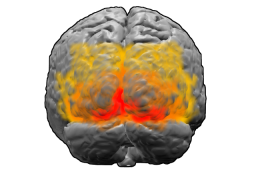
\includegraphics[width=1.0\textwidth]
          {./images/biological_inspirations/brodmann_areas_17_18_19.png}\\
          {\scriptsize 
          Rear view of the brain:\\
          Brodmann area 17 (red); area 18 (orange); area 19 (yellow).\\
          \color{col:attribution} 
          Image reproduced from \cite{Wikipedia:VisualCortex}}\\
         \end{center}
        \end{column}
        \begin{column}{0.62\textwidth}
            \vspace{0.2cm}
            \small
            The visual cortex includes several areas:
            \begin{itemize}
                \small
                \item The area that receives the sensory input is  
                 the \index{primary visual cortex}\gls{primary visual cortex}. 
                 It is also known as the
                 \index{visual area 1 (V1)} \gls{visual area 1 (V1)}, 
                 \index{Brodmann area 17} \gls{Brodmann area 17}, or 
                 \index{striate cortex} \gls{striate cortex}.
                \item
                 From V1, information is transmitted along 2 main pathways
                 to the the extrastriate cortex which consist of:
                 \begin{itemize}
                    \item Brodmann area 18, or visual area 2 (V2)
                    \item Brodmann area 19, or visual areas 3, 4 and 5 (V3-V5)
                \end{itemize}                    
            \end{itemize}                
        \end{column}
    \end{columns}


    \framebreak

    \index{CNN}\index{convolutional neural network}\glspl{cnn} 
    were inspired by studies of the 
    \index{primary visual cortex}\gls{primary visual cortex}
    of animals
    by T.Hubel and T.Wiesel\cite{Hubel:1959v1,Hubel:1962v1}.

    In a series of experiments, they studied the visual cortex by 
    \begin{itemize}
    \item {\bf projecting visual stimuli} on the 
      eyes of anaesthetized cats, and
    \item {\bf measuring the activity of neurons} by recording signals 
      on electrodes inserted in the brain.
    \end{itemize}

    \begin{columns}
        \begin{column}{0.55\textwidth}
            \begin{center}
            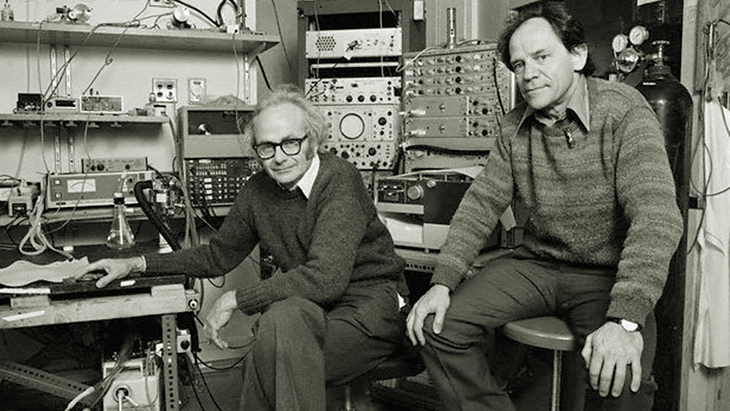
\includegraphics[width=0.9\textwidth]
                {./images/people/hubel_and_weisel.png}\\
            {\scriptsize 
            Hubel and Weisel.\\
            \color{col:attribution} 
            Photo from \cite{HarvardBrainTour:HubelAndWiesel}}\\
            \end{center}
        \end{column}
        \begin{column}{0.40\textwidth}
            \begin{center}
            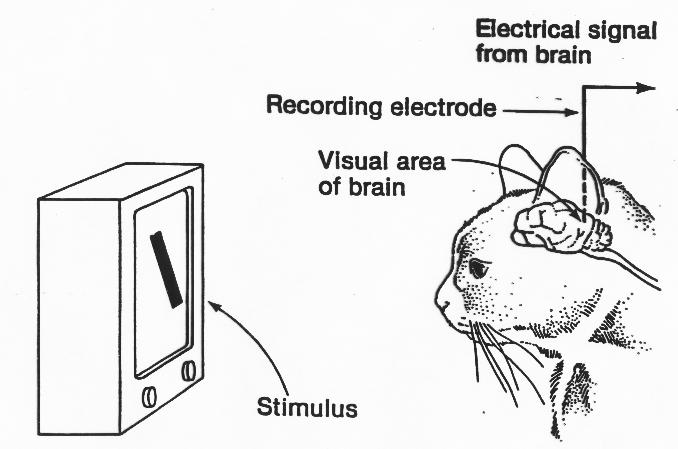
\includegraphics[width=1.0\textwidth]
                {./images/biological_inspirations/hubel_wiesel_experiment.png}\\
            {\scriptsize 
            Hubel and Wiesel experiment.\\
            \color{col:attribution} 
            Schematic from \cite{GoodPsychology:HubelAndWiesel}}\\
            \end{center}
        \end{column}
    \end{columns}


    \framebreak

    T.Hubel and T.Wiesel discovered that:
    \begin{itemize}
        \item Cells are arranged in columns.
        \item Colums are grouped together in hypercolumns, 
          each occupying a 2 mm x 2 mm area of the cerebral cortex.
        \item Each small area of the visual field is mapped to a hypercolumn.
        \item There are different types of cells:
        \begin{itemize}
            \item {\em Simple} cells responding best to elongated
               bars or edges of light or dark 
               that have a preferred orientation and location.
            \item {\em Complex} cells 
               receiving inputs from a collection of simple cells 
               with the same preferred orientation but 
               different preferred locations
        \end{itemize} 
    \end{itemize} 

    \begin{blockexample}{}
        \small
        T.Hubel and T.Wiesel were awarded the 1981 Nobel prize for Physiology.\\
        Details in \url{https://www.nobelprize.org/prizes/medicine/1981/}.
    \end{blockexample}

    \framebreak

    V1 performs a simple filtering to {\bf enhance edges and contours}.

\end{frame}


% Discuss the Neocognitron
\subsection{Convolutional Network precursors: Neocognitron}
%
%
%

\begin{frame}[t,allowframebreaks]{Convolutional Network precursors: Neocognitron -}

    In 1980, \index{Fukushima}\gls{Fukushima} 
    \cite{Fukushima:1980nc, Fukushima:1988nc, Fukushima:2019nc}, 
    inspired by the studies of the \index{primary visual cortex}\gls{primary visual cortex},
    created the \index{neocognitron}\gls{neocognitron}
    as a model of the visual system.\\
    \vspace{0.2cm}

    The \gls{neocognitron} is the precursor of the \gls{cnn}.\\
    \vspace{0.2cm}

    It is a hierarchical network consisting of many 
    stages of \index{neuron}\gls{neuron}-like cells
    preceded by an input layer U$_0$.\\
    \vspace{0.2cm}

    Each stage is composed of a layer of 
    {\bf S-cells} and a layer of {\bf C-cells}.
    \vspace{0.2cm}

    \begin{itemize}
        \item
        {\bf S-cells} behave like 
        \index{simple cell}\glspl{simple cell} in the 
        \gls{primary visual cortex}: 
        \begin{itemize}
            \item
            {\bf Feature extracting} cells 
            (i.e. respond selectively to specific features)
        \end{itemize}
        \item
        {\bf C-cells} behave like 
        \index{complex cell}\glspl{complex cell} in the 
        \gls{primary visual cortex}:
        \begin{itemize}
            \item Pool responses of S-cells with 
            different receptive fields 
            (i.e. perform a spatial averaging of S-cells response)\\
        \end{itemize}
    \end{itemize}
    \vspace{0.2cm}

    \framebreak

    Each layer of cells is divided into 
    sub-layers (\index{cell-plane}\glspl{cell-plane}).
    whose cells:
    \begin{itemize}
        \item respond to the same feature,
        \item are arranged retinotopically (each cell has a different receptive field) 
        \item share the same input connections
    \end{itemize}
    %\vspace{0.1cm}
    The input connections to S-cells are variable and modified during training.
    \begin{itemize}
        \item The {\bf features extracted by an S-cell are learned}.
        \item These are {\bf local features in shallow stages} and 
              more {\bf global features in deeper stages}.
    \end{itemize}
    %\vspace{0.1cm}
    The output of a layer of S-cells is fed to a layer of C-cells.
    \begin{itemize}
        \item Fixed set of connections, from extractors of same feature
            but with slightly different receptive fields
        \item C-cells pool the response of S-cells (spatial averaging); 
        Allows robust performance for deformed patters and noise suppression.
    \end{itemize}
    %\vspace{0.1cm}
    The output of the C-cells is fed into the next layer of S-cells.\\
    %The final classification is made in the deepest stage.

    \framebreak

    \begin{center}
        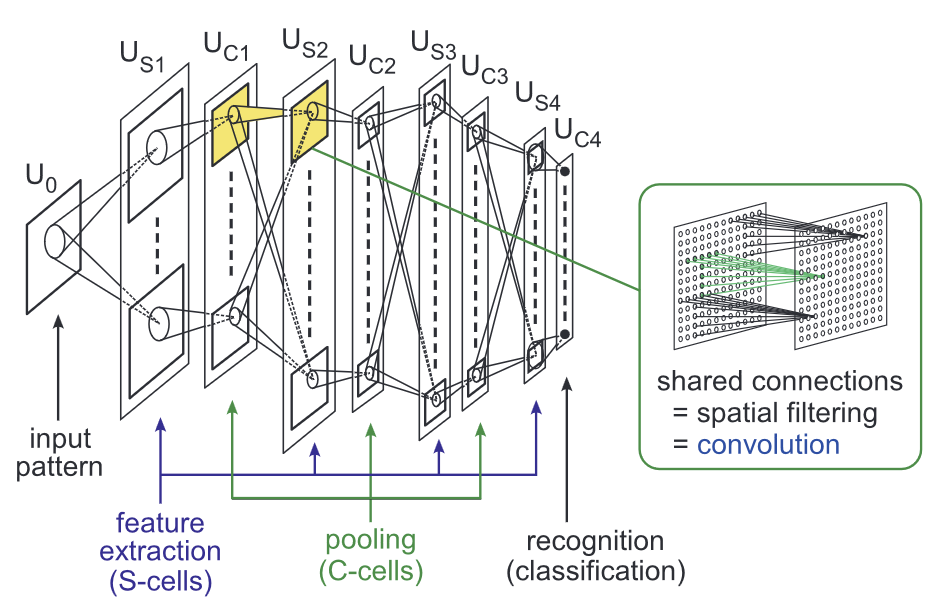
\includegraphics[width=0.80\textwidth]
           {./images/neocognitron/fukushima19_hierarchical_network_structure_01.png}\\
        {\scriptsize 
        Hierarchical network structure of the \gls{neocognitron}.\\
        $U_{S\ell}$($U_{C\ell}$) denotes the $\ell^th$ stage of S-cells (C-cells).
        $U_0$ is the input layer.\\
        \color{col:attribution} 
        Image reproduced from \cite{Fukushima:2019nc} (Fig.1)}\\
    \end{center}

    \framebreak

    \begin{columns}
        \begin{column}{0.55\textwidth}
            \begin{center}
                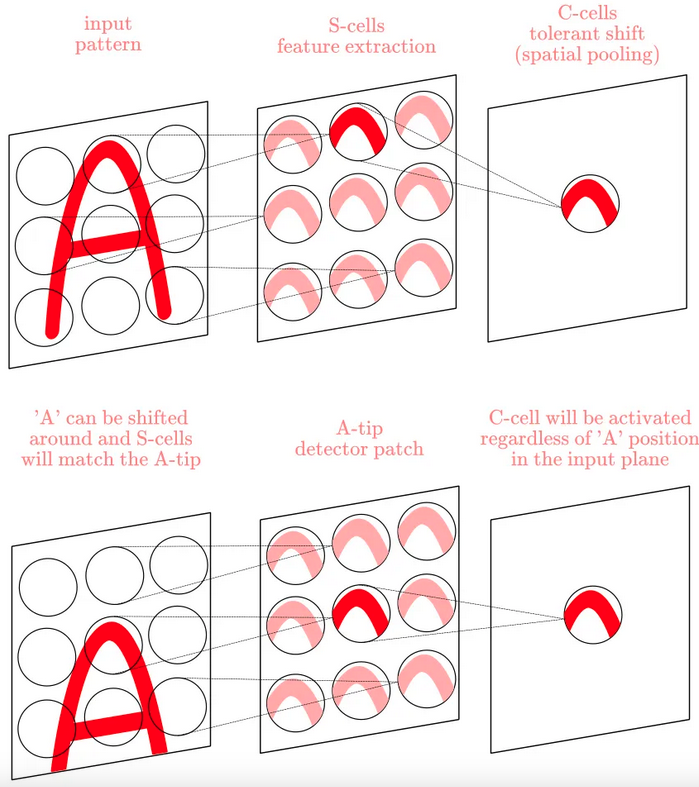
\includegraphics[width=0.90\textwidth]
                   {./images/neocognitron/elhamraoui20_feature_detection_schematic.png}\\
                {\scriptsize 
                \color{col:attribution} 
                Image reproduced from \cite{Medium:LeNet5andAlexNet}}\\
            \end{center}
        \end{column}
        \begin{column}{0.45\textwidth}
            \begin{center}
                Position-independence of feature detection in the \gls{neocognitron}.\\
            \end{center}
        \end{column}
    \end{columns}

\end{frame}




% Give a list of modern architectures, but defer detailed description 
% till after the basics of convolutional networks are described
\subsection{From the Neocognitron to modern convolutional architectures}
%
%
%

\begin{frame}[t,allowframebreaks]{From the Neocognitron to modern architectures -}

    The \index{neocognitron}\gls{neocognitron} 
    was an important development towards high-performing neural network
    architectures for computer vision.\\
    \vspace{0.2cm}
    Many key ideas are employed in modern architectures:    
    \begin{itemize}
        \item Creating a hierarchical network organisation
        \item Learning simple image features and combining them to produce more complex representations
    \end{itemize}
    \vspace{0.2cm}
    
    The \gls{neocognitron} 
    also differed from modern 
    \index{CNN}\index{convolutional neural network}\glspl{cnn}
    in important ways:
    \begin{itemize}
        \item Not using the backpropagation training method
        \item Not using weight sharing
    \end{itemize}

    \framebreak
    
    First fully convolutional architecture (\gls{LeNet-5}) was developed circa 2000.\\
    \vspace{0.2cm}
    Since then, \index{CNN}\index{convolutional neural network}\glspl{cnn}
    grew in prominence and achieved astonishing accuracy.\\
    \vspace{0.2cm}
    Indeed, \glspl{cnn} have been consistent winners
    of the \index{ILSVRC}\index{ImageNet}\gls{ilsvrc}.\\ 
    \vspace{0.2cm}
    Some well-known architectures are listed below:\\

    \begin{itemize}

        \item 
        \index{LeNet-5}\gls{LeNet-5}\cite{LeCun:1998ln5};
        First fully convolutional architecture 

        \item 
        \index{AlexNet}\gls{AlexNet}\cite{Krizhevsky:2012alexnet};
        Winner of \gls{ilsvrc} for 2012.
    
        \item 
        \index{ZFNet}\gls{ZFNet}\cite{Zaremba:2016zfnet};
        Winner of \gls{ilsvrc} for 2013.
    
        \item 
        \index{GoogLeNet}\gls{GoogLeNet} 
        (or \index{Inception}\gls{Inception} v1)
        \cite{Szegedy:2014gnet};
        Winner of \gls{ilsvrc} for 2014.
    
        \item 
        \index{VGG}\gls{VGG}\cite{Simonyan:2015vgg};
        A close second of \gls{ilsvrc} for 2014.
    
        \item 
        \index{ResNet}\gls{ResNet}\cite{He:2016resnet};
        Winner of \gls{ilsvrc} for 2015.    
    \end{itemize}

    \vspace{0.2cm}
    Some of these architectures will be discussed in detail later.
    
    \end{frame}
    


%
%
%

\subsection{The convolution and cross-correlation operations}
%
% Convolution and cross-correlation operations
%

\begin{frame}[t,allowframebreaks]{The convolution and cross-correlation operations -}

    A \index{convolution}\gls{convolution} is 
    a mathematical operation on two functions $f(x)$ and $g(x)$ of a real-valued argument $x$.\\

    \vspace{0.1cm}
    It produces a third function, denoted $(f \ast g)$, which is defined as:
    \begin{equation}
        (f \ast g) (x) = 
          \int_{-\infty}^{+\infty} 
            f(\alpha) g(x-\alpha) d\alpha
        \label{eq:convolution_cont1d_1}
    \end{equation}        

    Convolution is {\em commutative}: 
    \begin{equation}
        (f \ast g) (x) = (g \ast f) (x) 
        \label{eq:convolution_commutative_1}
    \end{equation}        
    
    Therefore, the following is an equivalent definition:
    \begin{equation}
        (f \ast g) (x) = 
          \int_{-\infty}^{+\infty} 
            f(x-\alpha) g(\alpha) d\alpha
        \label{eq:convolution_cont1d_2}
    \end{equation}        

    A \gls{convolution} is defined for any functions $f(x)$ and $g(x)$ 
    for which the above integrals 
    (Eqs. \ref{eq:convolution_cont1d_1} and \ref{eq:convolution_cont1d_2}) 
    are defined.\\

    \framebreak

    We often convolute $f(x)$ with a function $g(x)$ that has special properties, 
    to calculate a weighted average of $f(x)$ (e.g. a moving average).\\

    \begin{blockexample}{}
        \small
        For example, assume that:
        \begin{itemize}
            \small
            \item 
              $s(t)$ gives the closing price of a stock, 
              or the temperature at a specific location, as a function of time, and
            \item
              We want to remove noise from $s(t)$ to reveal long-term trends.          
        \end{itemize}
        We can achieve this with a weighting function $w(t^\prime)$,
        where $t^\prime$ is the time that has elapsed since a measurement:
        \begin{equation}
            (s \ast w) (t) = 
              \int_{-\infty}^{+\infty} 
                s(t-t^\prime) w(t^\prime) dt^\prime
            \label{eq:convolution_cont1d_low_pass_filter_1}
        \end{equation}
        The weighting function $w(t^\prime)$ must be a valid probability density function,
        with $w(t^\prime<0)=0$ to avoid including future values into the moving average.
    \end{blockexample}

    \framebreak

    \begin{columns}
        \begin{column}{0.45\textwidth}
         \begin{center}
            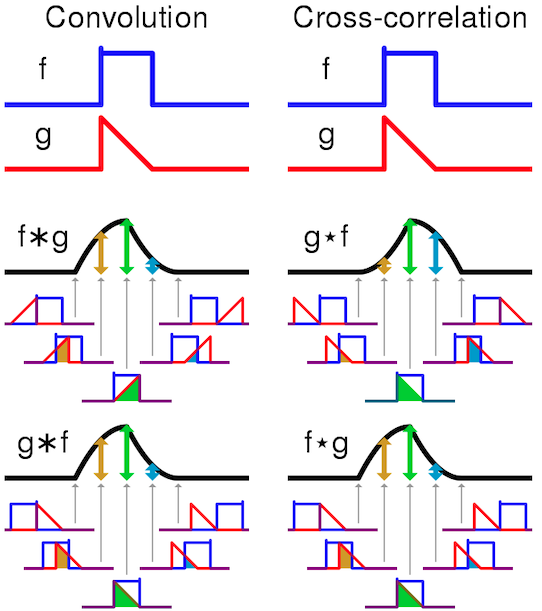
\includegraphics[width=0.99\textwidth]
            {./images/convolution/wikipedia_comparison_conv_corr_02.png}\\
         {\scriptsize 
          Comparison of convolution, cross-correlation.\\
          \color{col:attribution} 
          Image reproduced from \cite{Wikipedia:Convolution}}\\
          \end{center}
        \end{column}
        \begin{column}{0.55\textwidth}
            The \index{convolution}\gls{convolution} $(f \ast g) (x)$ of real-valued functions 
            $f(x)$ and $g(x)$ was defined in 
            Eqs. \ref{eq:convolution_cont1d_1} and \ref{eq:convolution_cont1d_2}.\\
            \vspace{0.2cm}
            % \begin{equation*}
            %     (f \ast g) (x) = 
            %       \int_{-\infty}^{+\infty} 
            %         f(\alpha) g(x-\alpha) d\alpha = 
            %       \int_{-\infty}^{+\infty} 
            %         f(x-\alpha) g(\alpha) d\alpha
            % \end{equation*}                
            A related mathematical operation of the 
            \index{cross-correlation}\gls{cross-correlation} $(f \star g) (x)$.\\
            \vspace{0.2cm}
            The \index{convolution}\gls{convolution} $(f \ast g) (x)$ differs from 
            \index{cross-correlation}\gls{cross-correlation} $(f \star g) (x)$
            in that, in \gls{convolution}, 
            either $f(x)$ and $g(x)$ are reflected about the y axis.\\
        \end{column}
    \end{columns}

    \framebreak

    Usually, we work with data where $x$ takes discrete values 
    and $f(x)$ is stored as an array.
    We can define a discrete \index{convolution}\gls{convolution} as:
    \begin{equation}
        (f \ast g) (i) = 
          \sum_{m} 
            f(m) g(i-m)
        \label{eq:convolution_disc1d_1}
    \end{equation}        

    Very often, our input data are multi-dimensional 
    and our definition of the \gls{convolution} operation needs to be extended accordingly.
    For example, for an image described by a two-dimensional array $f$,
    \gls{convolution} is defined as:
    \begin{equation}
        (f \ast g) (i,j) = 
          \sum_{m} \sum_{n} 
          f(m,n) g(i-m, j-n)
        \label{eq:convolution_disc2d_1}
    \end{equation}        

    In \index{convolutional neural network}\gls{cnn} literature,
    $f$ is often referred to as the input, 
    while $g$ is referred to as the kernel.

    \framebreak
   
    The discrete \index{convolution}\gls{convolution}
    of two-dimensional data was defined as:
    \begin{equation*}
        (f \ast g) (i,j) = 
          \sum_{m} \sum_{n}
          f(m,n) g(i-m, j-n)
        \label{eq:convolution_disc2d_1}
    \end{equation*}        

    Using the commutative property of the convolution, it can be rewritten as:
    \begin{equation}
        (f \ast g) (i,j) = 
          \sum_{m} \sum_{n}
          f(i-m,j-n) g(m, n)
        \label{eq:convolution_disc2d_2}
    \end{equation}        

    In practical applications, the latter expression 
    where the kernel $g$ is flipped relative to the input $f$ is easier to implement.
    \begin{itemize}
      \item The kernel has a smaller range than the input.\\
    \end{itemize}
    \vspace{0.2cm}

    Actually, many \gls{ml} libraries implement the following 
    \index{cross-correlation}\gls{cross-correlation}, but call it \gls{convolution}:
    \begin{equation}
        (f \star g) (i,j) = 
          \sum_{m} \sum_{n}
          f(i+m,j+n) g(m, n)
        \label{eq:cross_correlation_disc2d_1}
    \end{equation}        

    \framebreak

    \begin{center}
        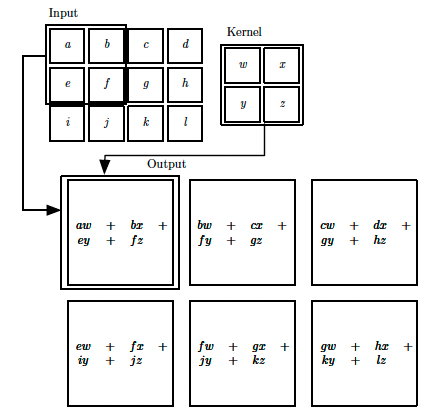
\includegraphics[width=0.60\textwidth]
        {./images/convolution/goodfellow17_convolution_2d_01.png}\\
     {\scriptsize 
      An example of 2-D convolution.\\
      \color{col:attribution} 
      Image reproduced from p.325 of \cite{Goodfellow:2017MITDL}}\\
    \end{center}

\end{frame}



\subsection{Motivation}
\begin{frame}[t,allowframebreaks]{Ad}

    \glspl{cnn} use \index{convolution} \gls{convolution}
    operations in at least one of their layers, instead of general matrix multiplication.

    As it is discussed in \cite{Goodfellow:2017MITDL} 
    (see Sec. 9.2 for a detailed discussion), \gls{convolution} 
    enables:
    \begin{itemize}
        \item Sparse connectivity
        \item Parameter sharing
        \item Equivariant representations
    \end{itemize}

\end{frame}

\subsubsection{Sparse connectivity}
\begin{frame}[t,allowframebreaks]{Sparse connectivity -}

    \begin{itemize}
        \item 
        In the fully connected neural networks described earlier in this module, 
        {\bf every output unit interacts with every input unit} 
    \end{itemize}

    \framebreak

    \begin{columns}
        \begin{column}{0.50\textwidth}
         \begin{center}
          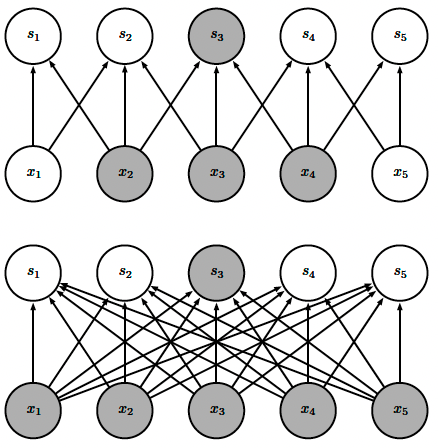
\includegraphics[width=1.0\textwidth]
          {./images/cnn/sparse_connectivity/goodfellow17_sparse_connectivity_from_above_01.png}\\
          {\scriptsize \color{col:attribution} 
          Image reproduced from p.327 of \cite{Goodfellow:2017MITDL}}\\
         \end{center}
        \end{column}
        \begin{column}{0.50\textwidth}
        \end{column}
    \end{columns}

    \framebreak

    \begin{columns}
        \begin{column}{0.50\textwidth}
         \begin{center}
          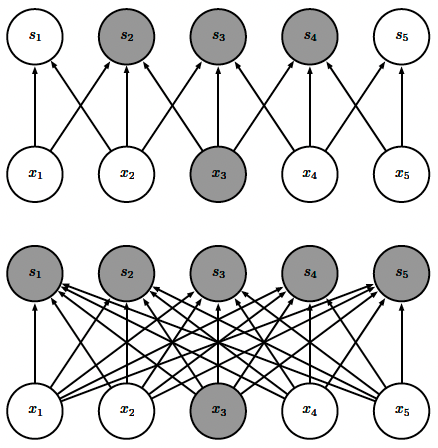
\includegraphics[width=1.0\textwidth]
          {./images/cnn/sparse_connectivity/goodfellow17_sparse_connectivity_from_below_01.png}\\
          {\scriptsize \color{col:attribution} 
          Image reproduced from p.327 of \cite{Goodfellow:2017MITDL}}\\
         \end{center}
        \end{column}
        \begin{column}{0.50\textwidth}
        \end{column}
    \end{columns}

\end{frame}

%
%
%

\begin{frame}[t,allowframebreaks]{Parameter sharing -}

\end{frame}

%
%
%

\begin{frame}[t,allowframebreaks]{Equivariant representations -}

\end{frame}

%
%
%

\begin{frame}[t]{Basic structure of a Convolutional Neural Network}

    Typically, a \index{CNN}\index{convolutional neural network}\gls{cnn} layer
    consists of {\bf 3 stages}:
    \begin{enumerate}
        \item {\bf Convolution} stage:
           Performing convolutions in parallel. 
           Linear activations           
        \item {\bf Detector} stage:
        \item {\bf Pooling} stage:
    \end{enumerate}

\end{frame}

\subsection{Case studies}


\subsubsection{LeNet-5}

\subsubsection{AlexNet}

\subsubsection{GoogLeNet}

\subsubsection{ResNet}
